% Teilauswertung 1

\section{Mittelung und Fouriertransformation}
\label{sec:mittelungAndTrafo}

\paragraph{a)}\textbf{Experimentelle Bestimmung der Fourierentwicklungskoeffizienten}\\
Im Folgendem wird die Fourierentwicklungskoeffizienten der Sinus, Rechteck und Dreiecksschwingung experimentelle bestimmt. Dazu werden die einzelnen Peaks im Fourierspektrum ermittelt, welche dann den Wert der Fourierentwicklungskoeffizienten für diese Frequenz darstellen. Beachtet werden nur ungerade Vielfache der eingestellten Frequenz. Dies folgt aus Kapitel \ref{sec:fourierseries} bei der nur ungerade Vielfache in der Reihenentwicklung von Rechteck und Dreieckschwingung vorkommen. Die Daten der Amplitude $A$ wurden dabei in deziBel aufgenommen. Für die Umrechnung der Amplitude in deziBel zu Volt wird die Gleichung (\ref{eq:spannungpegel}) aus Kapitel \ref{sec:pegel} auf Spannung $U$ umgewandelt und erhält:
\begin{gather}
    L_U = 20 \log_{10}\left(\frac{U}{U_0}\right)~\Leftrightarrow~U = U_0 \cdot 10^{\frac{L_U}{20}}
\end{gather}
Zu beachten ist noch, dass die Spannung $U$ die gemessene Effektivspannung ist mit dem Faktor aus Kapitel \ref{sec:fourierseries} umrechnen für die Sinusschwingung, da die Fourierreihe der jeweiligen Schwingung rein aus Sinusschwingungen besteht. Die verwendeten Formeln sind dann:
\begin{gather}
    U = U_0 \cdot 10^{\frac{L_U}{20}} \cdot \sqrt{2}    
    \label{eq:umrechnung}
\end{gather}
Die Auswertung ergibt dann Tabelle \ref{tab:fourierkoeff}, in welcher man gut erkennen kann, dass die gemessenen Werte nicht weit von der Theorie abweichen. Die größte Abweichung weißen dabei die Werte bei einer Frequenz von 1000Hz auf. Dies kann aufgrund des höheren Spannungspegels $L_U$ geschehen sein, da bei einem niedrigeren Spannungspegel bei höheren Frequenzen die Abweichung stetig abnimmt.
\newpage
\begin{center}
    \textbf{Sinus}\\[0,2cm]
    \begin{tabular}{l | c | c c}
        $k$ & $f$/kHz &   $A_{mess}$/V & $A_{Theo}$/V \\
        \hline
        1 & 1 &  1.0024 & 1.0000 \\
    \end{tabular}\\[0,5cm]
    \begin{tabular}{c c}
        \textbf{Rechteck} & \textbf{Dreieck} \\[0,2cm]
        \begin{tabular}{l | c | c c}
            $k$ & $f$/kHz  &   $A_{mess}$/V & $A_{Theo}$/V \\
            \hline
            1  &       1 &  1.276204 &  1.273240 \\
            2  &       3 &  0.425216 &  0.424413 \\
            3  &       5 &  0.254976 &  0.254648 \\
            4  &       7 &  0.181976 &  0.181891 \\
            5  &       9 &  0.141379 &  0.141471 \\
            6  &      11 &  0.115513 &  0.115749 \\
            7  &      13 &  0.097574 &  0.097942 \\
            8  &      15 &  0.084397 &  0.084883 \\
            9  &      17 &  0.074300 &  0.074896 \\
            10 &      19 &  0.066309 &  0.067013 \\
            11 &      21 &  0.059820 &  0.060630 \\
            12 &      23 &  0.054445 &  0.055358 \\
            13 &      25 &  0.049915 &  0.050930 \\
            14 &      27 &  0.046045 &  0.047157 \\
            15 &      29 &  0.042696 &  0.043905 \\
            16 &      31 &  0.039764 &  0.041072 \\
            17 &      33 &  0.037185 &  0.038583 \\
            18 &      35 &  0.034885 &  0.036378 \\
            19 &      37 &  0.032824 &  0.034412 \\
            20 &      39 &  0.030967 &  0.032647 \\
            21 &      41 &  0.029284 &  0.031055 \\
            22 &      43 &  0.027747 &  0.029610 \\
            23 &      45 &  0.026338 &  0.028294 \\
            24 &      47 &  0.025044 &  0.027090 \\
            25 &      49 &  0.023854 &  0.025984 \\
            26 &      51 &  0.022747 &  0.024965 \\
            27 &      53 &  0.021718 &  0.024023 \\
            28 &      55 &  0.020760 &  0.023150 \\
            29 &      57 &  0.019863 &  0.022338 \\
            30 &      59 &  0.019024 &  0.021580 \\
            31 &      61 &  0.018230 &  0.020873 \\
            32 &      63 &  0.017489 &  0.020210 \\
            33 &      65 &  0.016786 &  0.019588 \\
            34 &      67 &  0.016126 &  0.019004 \\
            35 &      69 &  0.015501 &  0.018453 \\
        \end{tabular} \hspace{0,5cm} &
        \begin{tabular}{l | c | c c}
            $k$ & $f$/kHz &  $A_{mess}$/V & $A_{Theo}$/V \\
            \hline
            1  &       1 &  0.812606 &  0.810569 \\
            2  &       3 &  0.090246 &  0.090063 \\
            3  &       5 &  0.032489 &  0.032423 \\
            4  &       7 &  0.016573 &  0.016542 \\
            5  &       9 &  0.009979 &  0.010007 \\
            6  &      11 &  0.006700 &  0.006699 \\
            7  &      13 &  0.004805 &  0.004796 \\
            8  &      15 &  0.003604 &  0.003603 \\
            9  &      17 &  0.002806 &  0.002805 \\
            10 &      19 &  0.002247 &  0.002245 \\
            11 &      21 &  0.001853 &  0.001838 \\
            12 &      23 &  0.001530 &  0.001532 \\
            13 &      25 &  0.001298 &  0.001297 \\
            14 &      27 &  0.001116 &  0.001112 \\
            15 &      29 &  0.000963 &  0.000964 \\
            16 &      31 &  0.000846 &  0.000843 \\
            17 &      33 &  0.000737 &  0.000744 \\
            18 &      35 &  0.000654 &  0.000662 \\
            19 &      37 &  0.000591 &  0.000592 \\
            20 &      39 &  0.000521 &  0.000533 \\
            21 &      41 &  0.000480 &  0.000482 \\
            22 &      43 &  0.000433 &  0.000438 \\
            23 &      45 &  0.000395 &  0.000400 \\
            24 &      47 &  0.000362 &  0.000367 \\
            25 &      49 &  0.000335 &  0.000338 \\
            26 &      51 &  0.000312 &  0.000312 \\
            27 &      53 &  0.000280 &  0.000289 \\
            28 &      55 &  0.000264 &  0.000268 \\
            29 &      57 &  0.000255 &  0.000249 \\
            30 &      59 &  0.000237 &  0.000233 \\
            31 &      61 &  0.000218 &  0.000218 \\
            32 &      63 &  0.000205 &  0.000204 \\
            33 &      65 &  0.000194 &  0.000192 \\
            34 &      67 &  0.000181 &  0.000181 \\
            35 &      69 &  0.000170 &  0.000170 \\
        \end{tabular}
    \end{tabular}    
    \captionof{table}{Vergleich Fourierentwicklungskoeffizienten in Theorie und Praxis}
    \label{tab:fourierkoeff}
\end{center}
\paragraph{b)}\textbf{Fourierspektrum Sinusschwingung}\\
Dieser Teil behandelt das Fourierspektrum der Sinusschwingung bei 1V Amplitude.
\begin{center}
    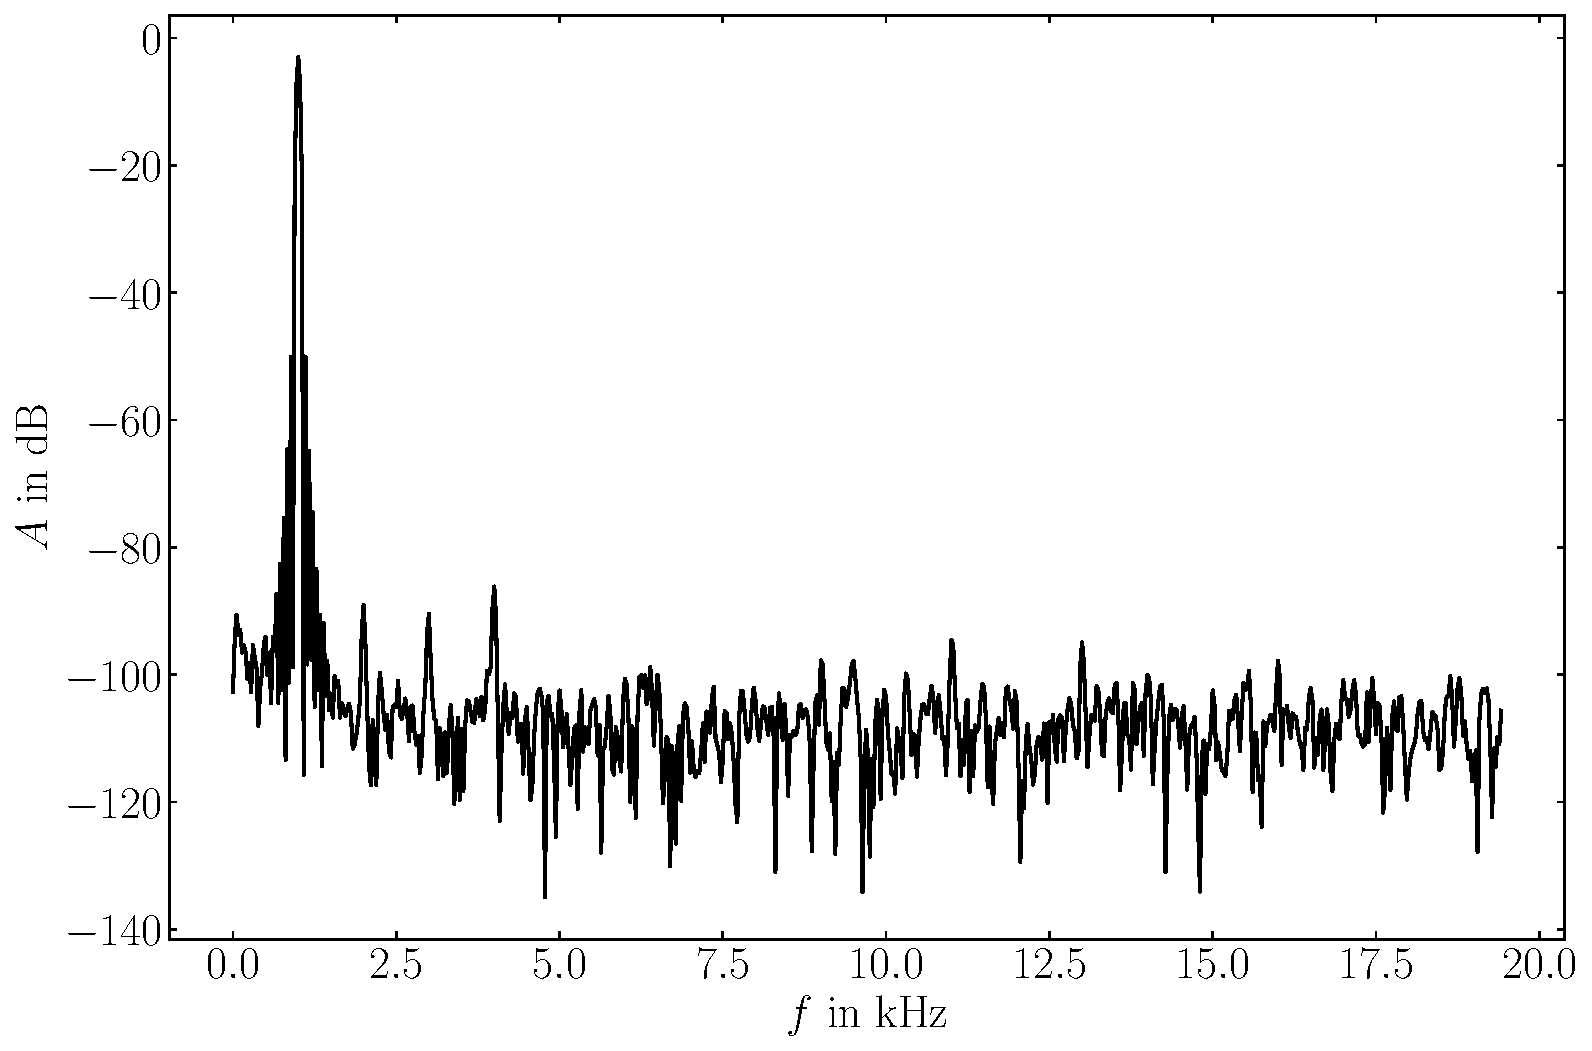
\includegraphics[scale = 0.5]{Manuel/41/FourierSinus.pdf}
    \captionof{figure}{Fourierspektrum der Sinusschwingung}
    \label{image:fourierSinus}
\end{center}
Wie in Abbildung \ref{image:fourierSinus} ist deutlich ein ausgeprägter Peak zu erkennen. Dieser Peak ist wie in Tabelle \ref{tab:fourierkoeff} die Effektivspannung der Sinusschwingung in deciBel. Nach Kapitel \ref{sec:fourierseries} sollte aber das Fourierspektrum nur einen Peak bei der eingestellten Frequenz besitzen, aber in Abbildung \ref{image:fourierSinus} ist neben dem Peak deutlich noch weiter Peaks zu erkennen. Diese Peaks werden durch die Umgebungseinflüsse aus Kapitel \ref{sec:umwelt} und durch die Netzspannungsquelle selbst verursacht.
\newpage
\paragraph{c)}\textbf{Einfluss Mittelung auf Rechteckschwingung}\\
Nun wird der Einfluss der Anzahl der Mittelung $N$ auf eine Rechteckschwingung mit einer Amplitude $U_0=$ 1V mit einem Bandrauschen der Bandbreite $f_{Band}=$ 20MHz und einer AM Depth $d =$ 120\% betrachtet.
\begin{center}
    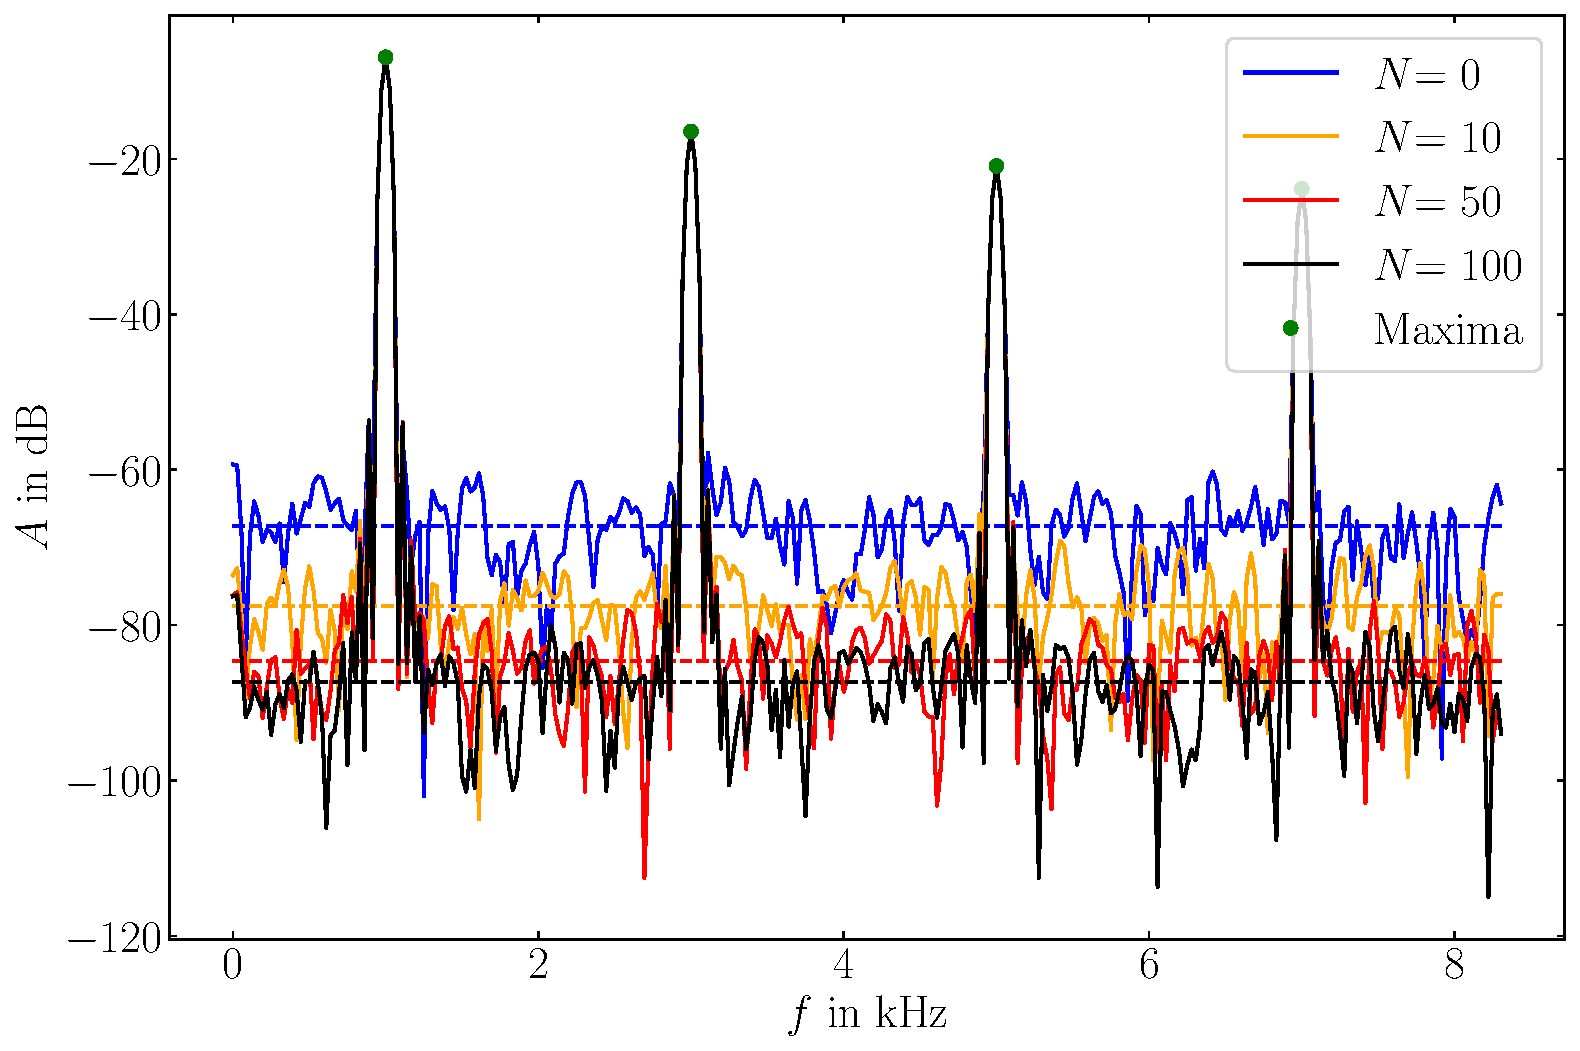
\includegraphics[scale = 0.5]{Manuel/41/Mittelung.pdf}
    \captionof{figure}{Einfluss der Mittelung auf Fourierspektrum einer Rechteckschwingung}
    \label{image:einflussMittelung}
\end{center}
In Abbildung \ref{image:einflussMittelung} ist zu erkennen, dass sich mit der Zunahme der Anzahl der Mittelungen $N$ die Ausprägung der Peaks zunimmt. Dies war zu erwarten, da schon wie in Kapitel \ref{sub:mittelung} erklärt, bei der Mittelung das Signal des Rauschens nur um den Faktor $\sqrt{N}$ zunimmt, während das Signal der Rechteckschwingung proportional zur Wiederholung anwächst.

\paragraph{d)}\textbf{Einfluss Signal/Rausch-Abstand auf zeitliche Signalform}\\
Als weiteres wird der Einfluss des Signal/Rausch-Abstands $d$ auf die Signalform einer Rechteckschwingung mit einer Amplitude $U_0=$ 1V und einen Bandbreite $f_{Band}=$ 20MHz.
In Abbildung \ref{image:sigRauRechtKomplett} ist zuerst der Einfluss des Signal/Rausch-Abstands auf die komplette Rechteckschwingung dargestellt. Schon hier erkennt man, dass mit höherem Signal/Rausch-Abstands das \enquote{Ausschlagen} der Amplitude des Rauschens zunimmt. Noch deutlich ist dies zu erkennen in Abbildung \ref{image:sigRauRecht}, die ein Ausschnitt aus dem oberen Umkehrpunkt der Rechteckschwingung ist. Die Änderung des Signal/Rausch-Abstands hat aber keinen generellen Einfluss auf den Verlauf der Signalform der Rechteckschwingung.
\newpage
\begin{center}
    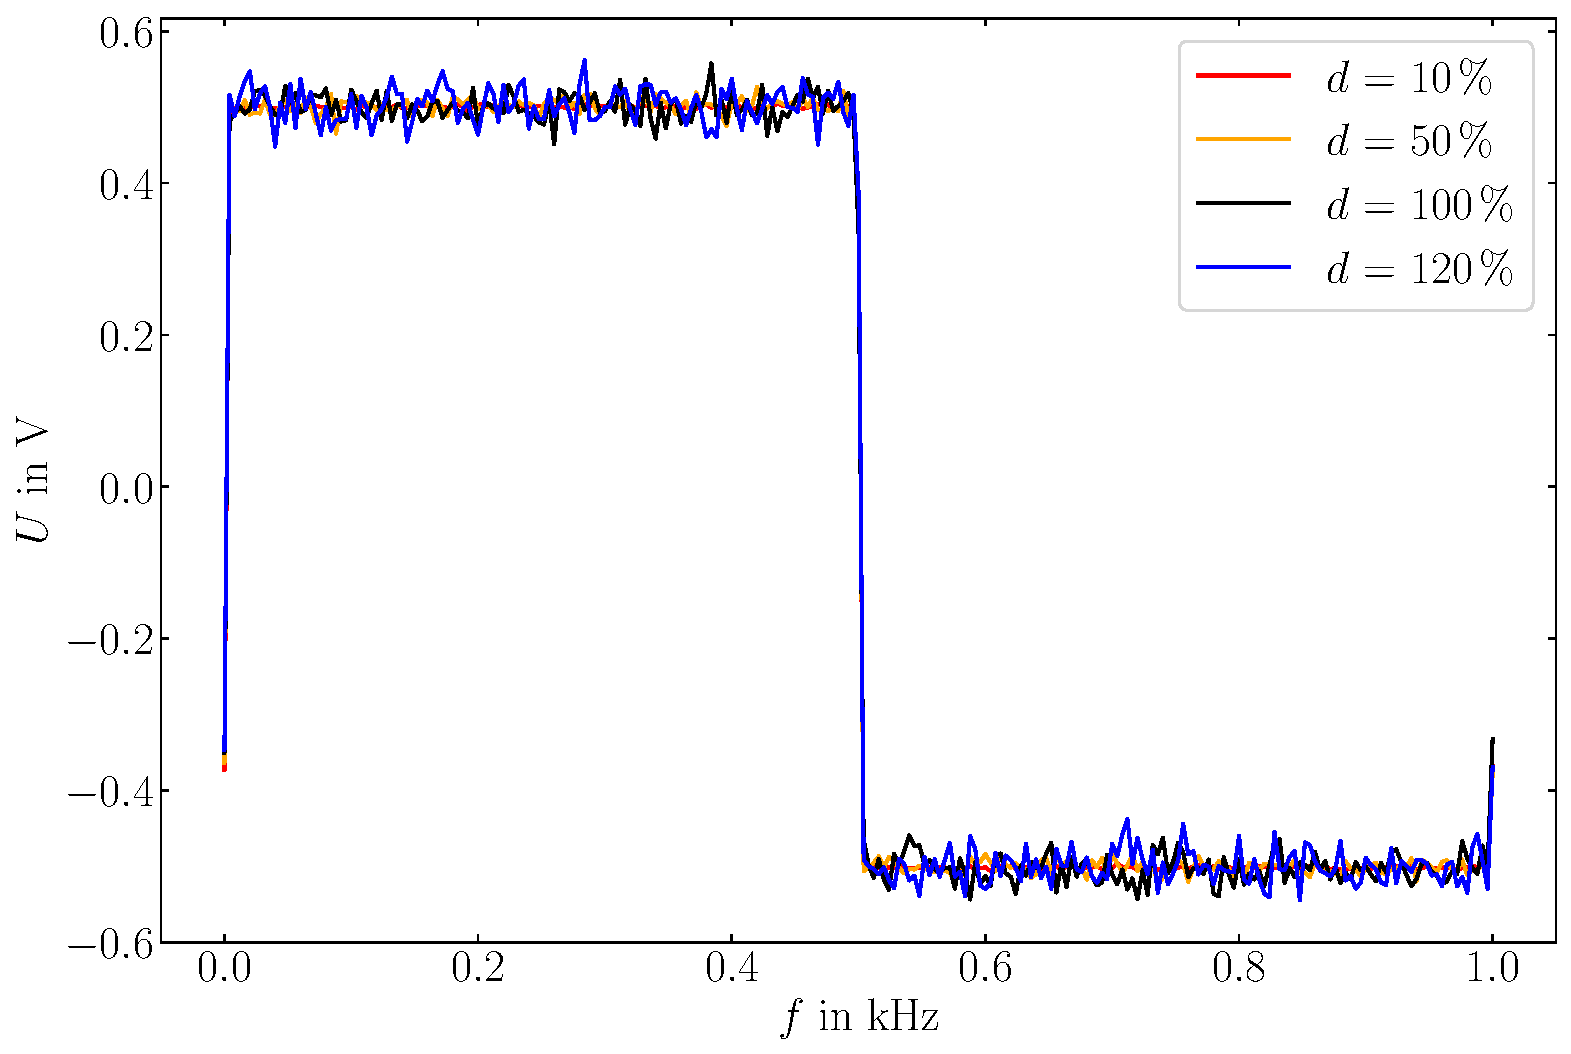
\includegraphics[scale = 0.5]{Manuel/41/SignalRauschAbstandKomplett.pdf}
    \captionof{figure}{Einfluss Signal/Rausch-Abstand auf komplette Rechteckschwingung}
    \label{image:sigRauRechtKomplett}
\end{center}
\begin{center}
    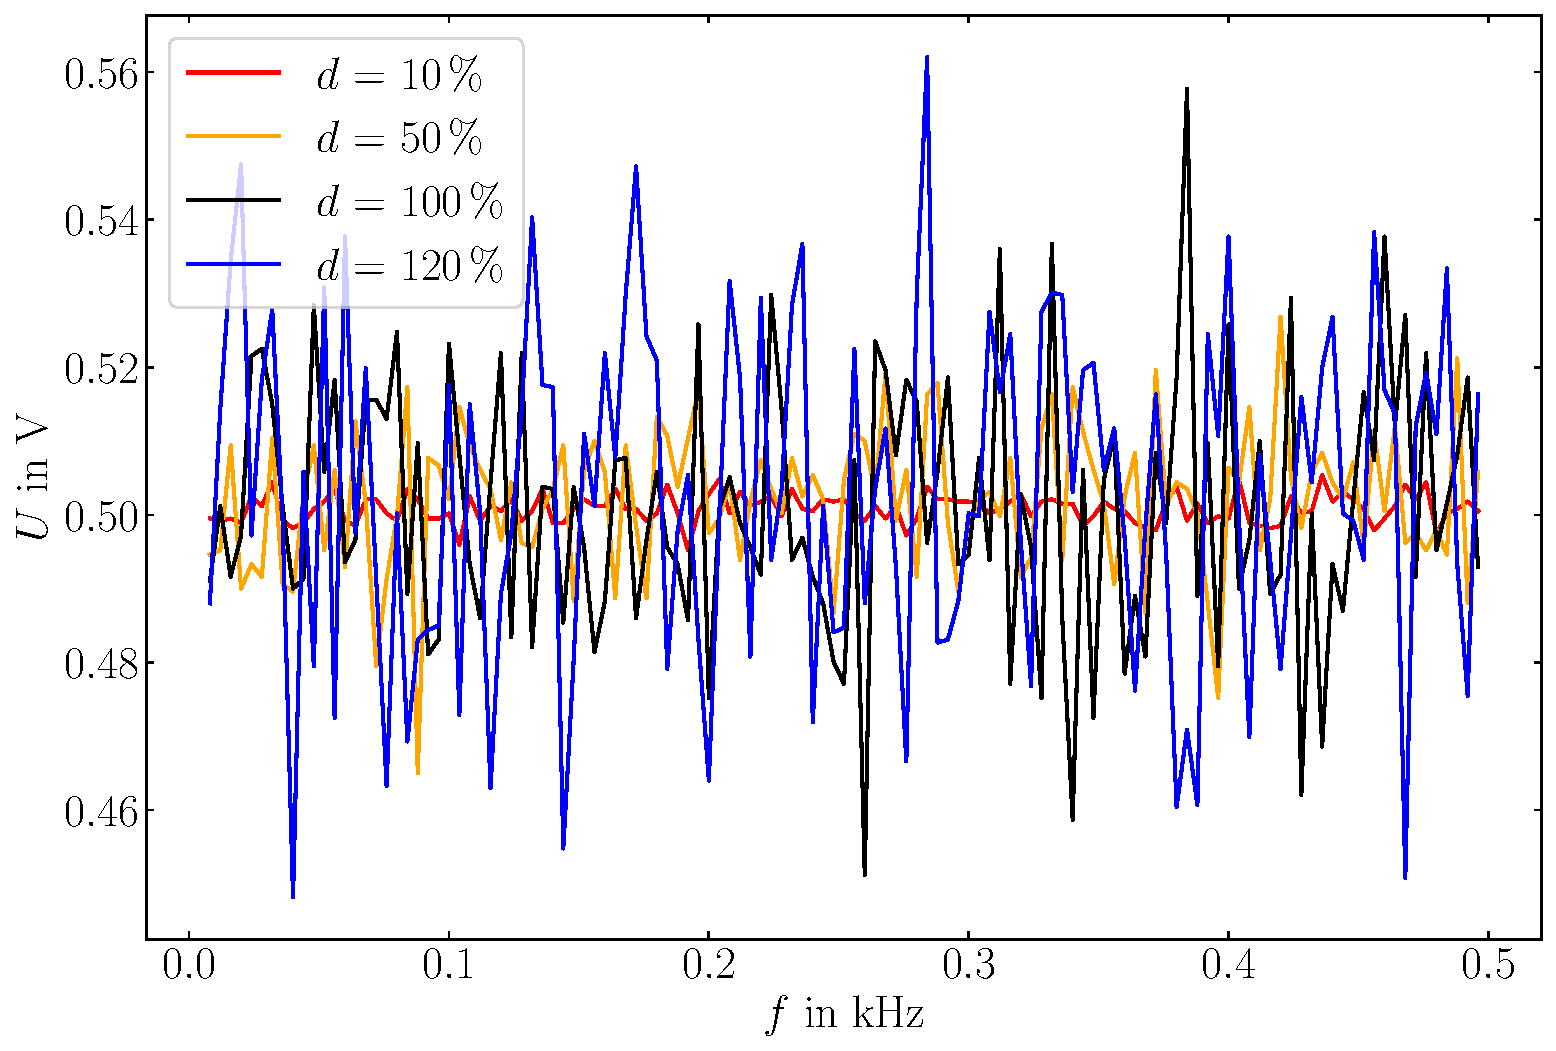
\includegraphics[scale = 0.5]{Manuel/41/SignalRauschAbstand.pdf}
    \captionof{figure}{Einfluss Signal/Rausch-Abstand im Ausschnitt vom obere Umkehrpunkt der Rechteckschwingung}
    \label{image:sigRauRecht}
\end{center}

\paragraph{e)}\textbf{Einfluss Bandbreite auf zeitliche Signalform}\\
Zuletzt in diesem Kapitel wird der Einfluss der Bandbreite auf die zeitliche Signalform besprochen. Dabei wird wieder eine Rechteckschwingung mit einer Amplitude $U_0=$ 1V und einem Signal/Rausch Abstand $d=$ 100\% verwendet. In Abbildung \ref{image:bandbreiteRechtKomplett} wird erneut eine komplette Rechteckschwingung gezeigt. Darauf erkennt man, dass der Funktionsgenerator die Form des Rechtecksignals mit kleineren Bandbreiten $f_{Band}$ nicht mehr erzeugen kann. Vor allem bei Frequenzen unter 100kHz. Aber auch eine Zunahme des Rauschens ist zu erkennen, wenn die Bandbreite kontinuierlich abnimmt. In Abbildung \ref{image:bandbreiteRecht} kann man dies noch genauer betrachten. 
\newpage
\begin{center}
    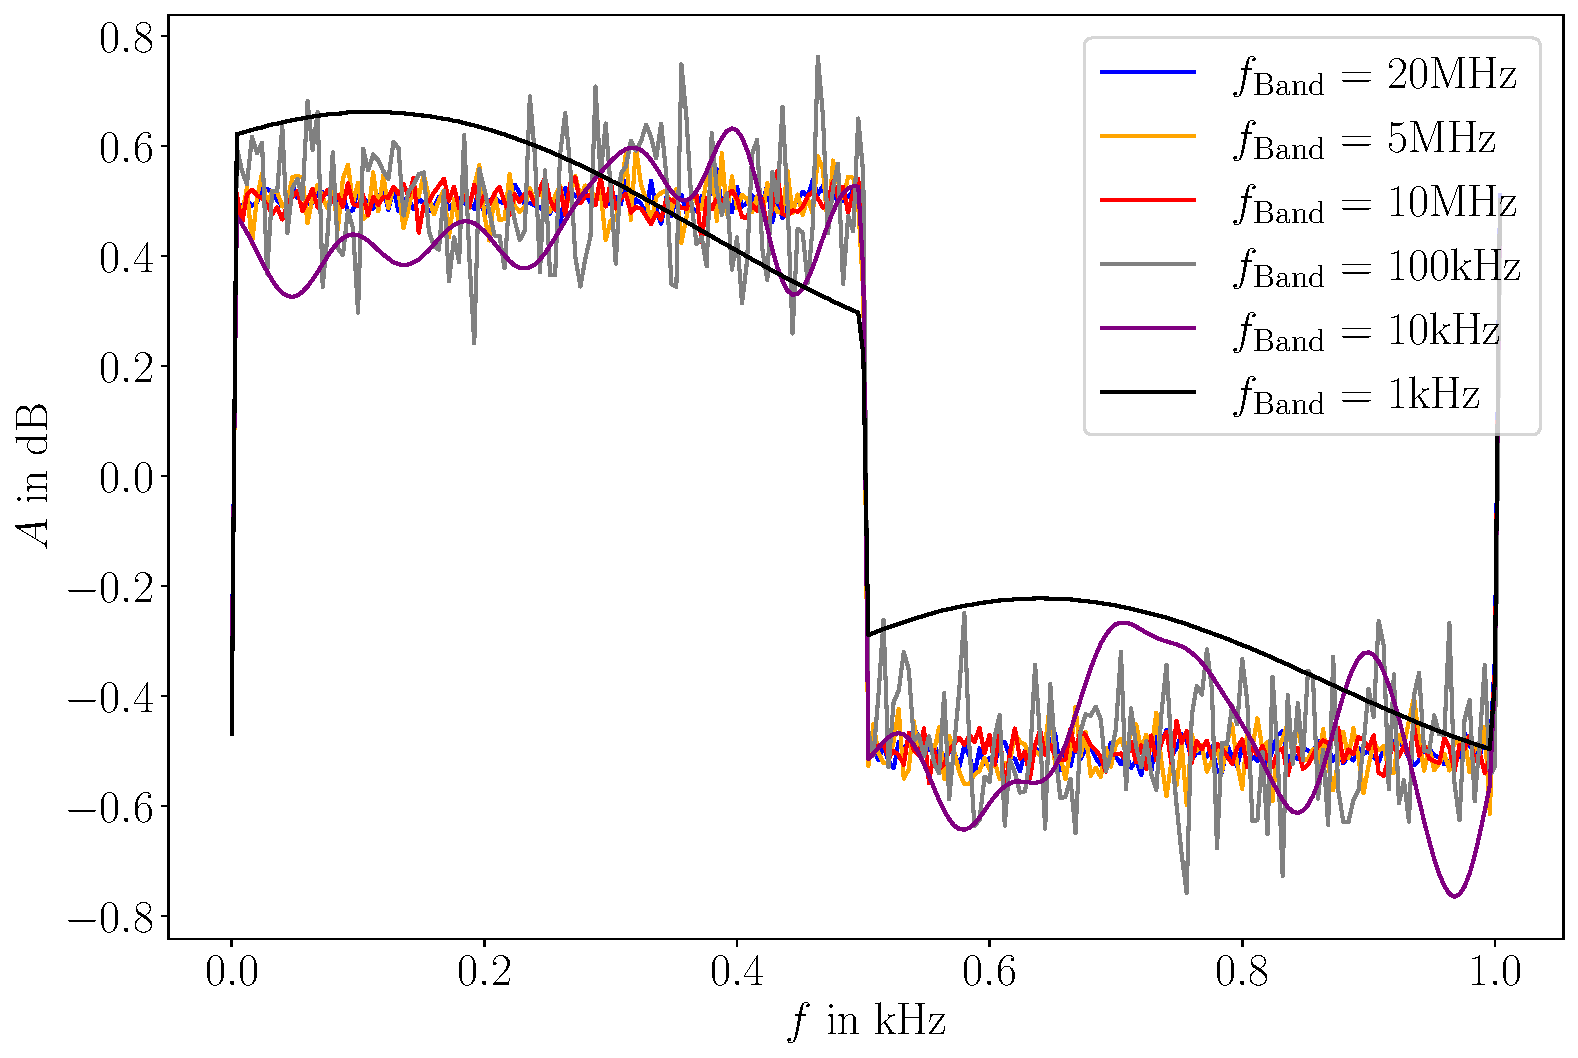
\includegraphics[scale = 0.5]{Manuel/41/BandbreiteKomplett.pdf}
    \captionof{figure}{Einfluss Bandbreite auf komplette Rechteckschwingung}
    \label{image:bandbreiteRechtKomplett}
\end{center}
\begin{center}
    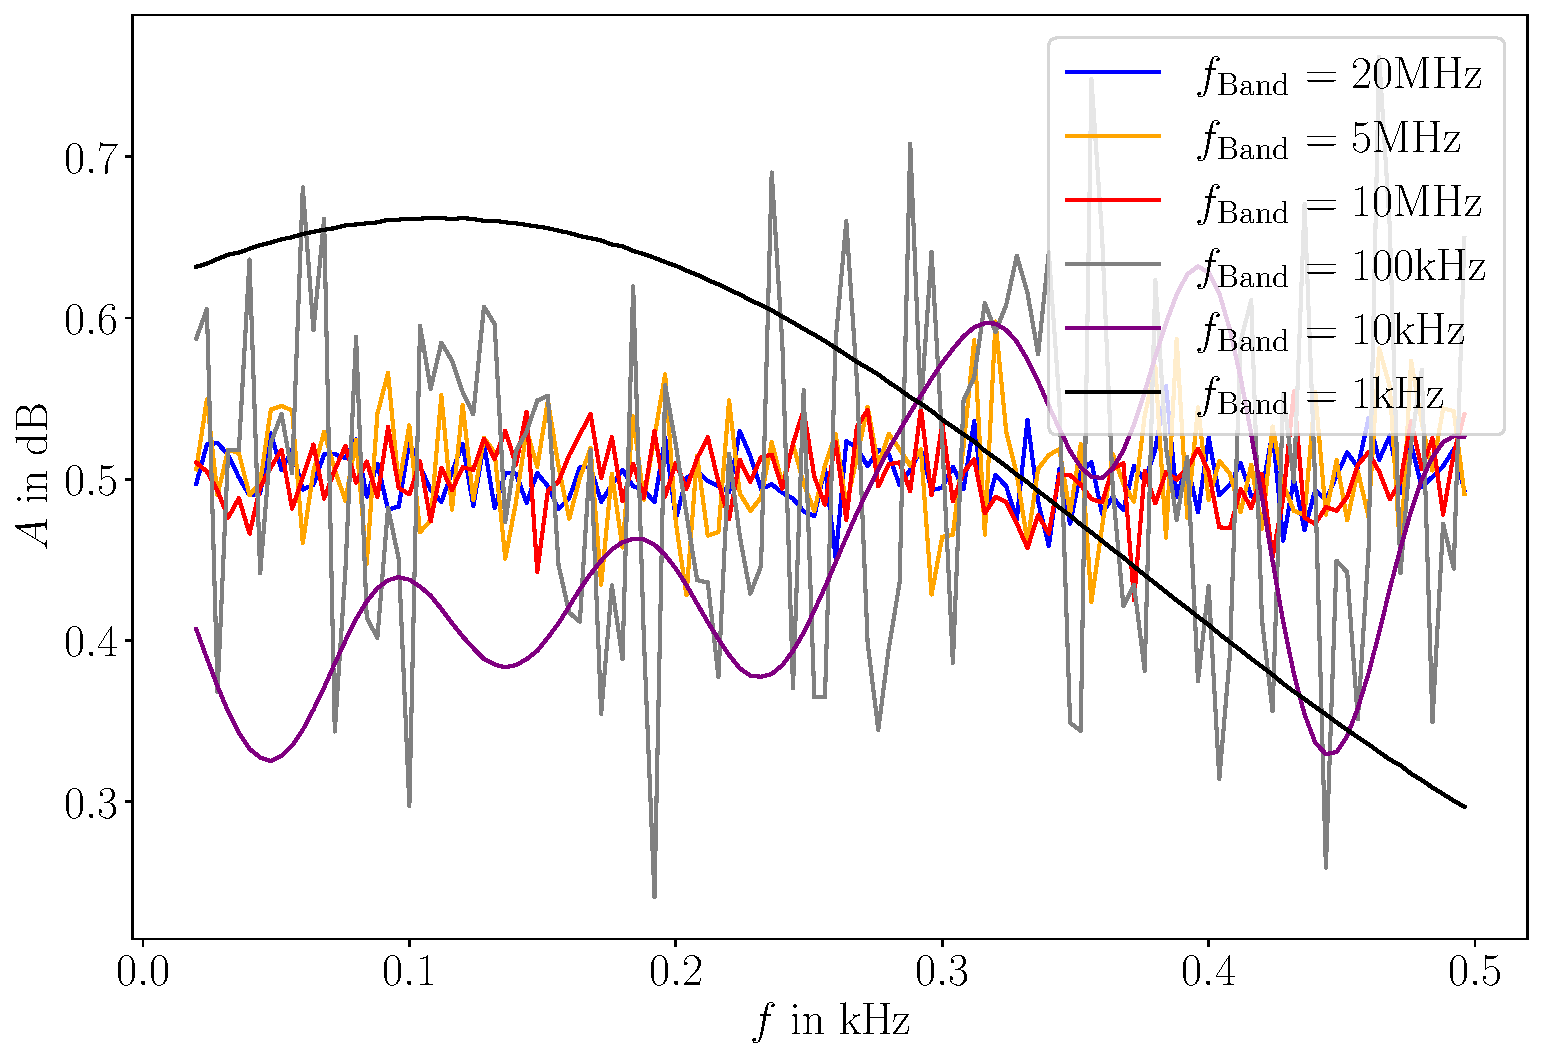
\includegraphics[scale = 0.5]{Manuel/41/Bandbreite.pdf}
    \captionof{figure}{Einfluss Bandbreite im Ausschnitt vom obere Umkehrpunkt der Rechteckschwingung}
    \label{image:bandbreiteRecht}
\end{center}